\documentclass[12pt, a4paper]{book}
\begin{document}
Machine Learning (ML) has emerged as a powerful tool for analyzing complex datasets and making accurate predictions. Its applications span across various fields, from natural language processing to image recognition, and it has been used successfully to solve a range of problems. \\
\\The main approach of this thesis will be to use ML as its popular rise has proven to be effective at binary classification tasks \cite{Baldi_2016, DeepLearing} in High Energy Particle Physics. 
For our purposes it will be a powerful tool to attempt to classify events as SM background or as DM signal.\\
\\To give a a short description of the essence of ML we can start by considering a general parameter $\bm{\beta} = \{\beta_1,\beta_2,\cdots,\beta_n\}$ for a n-dimensional problem, which for our purposes can be seen as what are called \textit{weights} and \textit{biases} 
($\bm \beta = \{w, b\}$), 
the goal is to choose these parameters $\bm{\beta}$ such that we minimize a cost (also called loss) function $C(\bm{\beta})$ with respect to a set of data points given by a matrix $\mathbf{X}$. This matrix $\mathbf{X}$ will be 
our dataset containing $n$ \textit{features} for each event $m$, and is of the following form 
\begin{equation}\label{eq:dataset}
    \bf X = \begin{pmatrix}
        x_{11} & x_{21} & x_{31} & \cdots & x_{n1}\\
        x_{12} & x_{22} & x_{32} & \cdots & x_{n2}\\
        x_{13} & x_{23} & x_{33} & \cdots & x_{n3}\\
        \vdots & \vdots & \vdots & \cdots & \vdots\\
        x_{1m} & x_{2m} & x_{3m} & \cdots & x_{nm}\\  
    \end{pmatrix}    
\end{equation}
This project will only focus on Supervised Learning, meaning that we know what the output is a binary representation of signal and background, such that we can use target values $\bm{t}$. 
Then we give the network a score depending on how close the predicted output is to real values $\bm t $. Then we repeat the process after tweaking the parameters $\bm \beta $ and see if the score gets better.\\
\\To this end, we will first provide a mathematical foundation for ML, starting with a brief overview of the different types of ML algorithms we will study, such as Neural Networks (NN) and Boosted Decision Trees (BDT). 
Other aspects such as the importance of feature selection and feature engineering in preparing the data for ML algorithms, as well as the concept of model evaluation and optimization will be discussed in Chapter \ref{chap:Method_ML}.


\newpage
\section{Neural Networks}\label{sec:theory_nn}
The theoretical foundation for this chapter is mainly based of Hjort-Jensen lecture notes \cite{MORTYY1, MORTYY2, MORTYY3}. Before begining we can briefly explain the idea behind NNs. As stated by Hjorth-Jensen in \cite{MORTYY1}:
\begin{quote}
    \textit{The idea of NN is to to mimic the neural networks in the human brain, which is composed of billions of neurons that communicate with each other by sending electrical signals. 
    Each neuron accumulates its incoming signals, which must exceed an activation threshold to yield an output. If the threshold is not overcome, the neuron remains inactive, i.e. has zero output}
\end{quote}
That takes us to what a \textit{neuron} is.


\subsection{Artificial neurons}\label{sec:neurons}
To describe the behaviour of a neuron mathematically we can use the following model that mimics how one neuron works
\begin{equation}\label{eq:neurons}
    y=f\left(\sum_{i=1}^{n}w_ix_i\right)=f(z)
\end{equation}
Where $y$, the output of the neuron, is the value of its \textit{activation function} (See section \ref{sec:act}), which has the weighted, $w_i$, sum of signals $x_i,\cdots,x_n$ received by $n$ neurons that are in a preciding layer.\\
\\The goal of NNs is to mimic the biological nervous system by letting each neuron interact with each other by sending signals, for us is in the form of a mathematical function between each layer, callled the activation function. 
Most NNs consist of an input layer, an output layer and intermediate layers, called hidden layers. All the layers can contain an arbitrary number of neurons, and each connection between two neurons is associated with a weight variable $w_i$.
The goal of using NNs is to teach the network the patterns of the data to then predict some target. In the context of our search for DM, by giving a NN our data set of events as its input layer, we can then train the network to classify events as signal or background.\\
\\Explained in greater detail if we were to look at a single event of the data, we start with an input with all the relevant features of the event, $\bm X$. Using Eq. (\ref{eq:neurons}) on every neuron on the next layer we can teach the network if there 
are any connections between the features, we can repeat this process for \textit{n} layers. As an output we want a single neuron to see if it has predicted the event to be a signal or background, since this is binary output. After analysing the prediction we can use the labels on the target data $\bm t$ 
to tell (the network) whether it predicted correctly or wrong. We can then use a \textit{cost function} and a specific \textit{metric} to evaluate numerically how well the network predicted the output by giving it a score. 
Seeing how the results fare we can then back-propagate to shift the weights and biases and repeat the process until we are satisfied with our result. Each of these iterations is called an epoch.\\
\\To generalize our artificial neuron to a whole network we can look at a Multilayer Perceptron (MLP). An MLP is a network consisting of at least three layers of neurons, the input, one or more hidden layers, and an output. 
The number of neurons can vary for each layer. The above explanation is a very dense and simplified one. In reality it is complicated to find out which cost function, activation function, metric, etc. are best suited to the given problem. 
But before we get into the gory details we can explore the mathematical model that illustrates what was tried to be explained above. 

\subsection{Optimizers}\label{sec:SGD}
The way we "tweak the parameters $\bm \beta $ to see if the network prediction gets better" is by using something called an \textit{optimizer}. We will mainly focus on the theory behind the \textit{Stochastic Gradient Descent} (SDG) optimizer as it is more easy to digest. Before explaining the SDG we have to look at the Gradient Descent (GD). \\
\\Given a cost function $C(\bm{\beta})$ we can get closer to the minimum by calculating the gradient $\nabla_{\beta}C(\bm{\beta})$ wrt. the unknown parameters from the NN $\bm\beta$. If we were to calculate the gradient at a specific 
point $\bm{\beta}_i$ in the parameter space, the negative gradient would correspond to the direction where a small change $d\bm\beta$ in this parameter space would result in the biggest decrease in the cost function. 
In the same way we in physics would determine where the local (or global) minima at a complex multidimensional potential numerically. In GD we can chose (which needs to be optimized) a step size $\eta$ related to the size of an iteration in the parameter space; 
this is called the \textit{learning rate}. The mathematical function for an iteration in parameter space to optimize the parameter $\bm{\beta}$ such that it minimizes the cost function is given as
\begin{equation}\label{eq:GD}
    \bm{\beta}_{i+1}=\bm{\beta}_{i} -\eta\nabla_{\beta}C(\bm{\beta}_i)
\end{equation}
To converge towards a minimum we should select a learning rate $\eta$ small enough to not "step over" the minimum point of the cost-function-space, but also not too small to get stuck on a local minimum rather than the global minimum. 
Thus using the learning rate as a hyperparameter in a grid search is a good way to optimize a NN for a given task.\\
\\In GD one computes the cost function and its gradient globally for all data points. This quickly becomes computationally heavy when dealing with large datasets. Thus a common approach is to compute the gradient over batches of the data. 
For our purposes it would be optimal to use GD, but our data size is massive, of the order of $10^{8}$ events (13 GB), becoming comupationally impossible. Thus instead of making a $n\times10^8$ matrix (see Eq. (\ref{eq:dataset})), 
we could for example split it into ten smaller matrices of $n\times10^7$ to then perform a parameter update, making the computation possible. This is where SGD comes in, for each step, or epoch the data is divided randomly into 
\textit{N} batches of size \textit{n}. Then for each batch we use Eq. (\ref{eq:GD}) to update the parameters, thus updating $\bm{\beta}_{i+1}$ \textit{N}-times for each epoch. The idea of SGD comes from the observation that the 
cost function can almost always be written as a sum over \textit{n} data points. The main advantage of SGD is not to ease the computation however, as using more batches also reduces the risk of getting stuck in a local minimum since it introduces a randomness of which part of the parameter space we move through, 
but this is at the cost of reducing statistics which might not be ideal for every problem.\\
\\There are other optimization algorithms we could use, such as the popular ADAM \cite{kingma2017adam}. The Adaptive Moment Estimation (ADAM) is a more advanced optimization algorithm that uses adaptive learning rates. It computes individual learning rates for each weight based on the average of past gradients 
and their variances. ADAM also uses momentum to accelerate the convergence of the optimization algorithm. We will test both ADAM and SGD when optimizing our networks.

\subsection{Activation functions}\label{sec:act}
As seen in Section \ref{sec:neurons}, an important aspect of NNs are activation functions and cost functions. As shall become apparent in Section \ref{sec:FFN}, when evaluating an activation function we get the neuron output, but what are these activation functions? 
Mathematically speaking, activation functions are: Non-constant, Bounded, Monotonically-increasing and continuous functions. In this project we will utilize two different activation functions at different layers. 
The first one is a sigmoid activation function
\begin{equation}\label{eq:sig}
    f(x) = \frac{1}{1+e^{-x}}
\end{equation}
which is the most basic activation function, this will be used from the input layer to our fist hidden layer as the risks of having little neuron activation is minimal here. On all other layers I will utilise a Rectified Linear Unit (ReLU)
\begin{equation}\label{eq:ReLU}
    f(x) = x^+ = \text{max}(0,x) = \begin{cases}x&{\text{if }}x>0,\\0.&{\text{otherwise}}.\end{cases}
\end{equation}
which has better gradient propagation, meaning that there are fewer vanishing gradient problems compared to the sigmoidial function.


\subsection{Feed Forward network}\label{sec:FFN}
To describe how the network "guesses" outputs in a mathematical model we can start by looking at Eq. (\ref{eq:neurons}) where we got an output $y$ from an activation function $f$ that receives $x_i$ as input. 
We can expand the function as as following
\begin{equation}\label{eq:activation}
    y=f\left(\sum_{i=1}^nw_ix_i+b_i\right)=f(z)
\end{equation} 
where $w_i$ is still the weight and we now use the previously introduced bias $b_i$ which is normally needed in case of zero activation weights or inputs. The difference comes now in the interpretation; where in the activation 
$z=(\sum_{i=1}^nw_ix_i+b_i)$ the inputs $x_i$ are now the outputs of the neurons in the preceding layer. Furthermore an MLP is fully-connected, meaning that each neuron received a weighted sum of the output of \textbf{all} 
neurons in the previous layer. To expand Eq. (\ref{eq:activation}) we can first look at the output of every neuron $i$ in a weighted sum $z^1_i$ for each input $x_j$ on a layer
\begin{equation}\label{eq:weightedsum}
    z_i^1=\sum_{j=1}^Mw_{ij}^1x_j + b^1_i
\end{equation}
Where $M$ stands for all possible inputs to a given neuron $i$ in the \textit{first} layer. Such that if we evaluate the weighted sum in an activation function $f_i$ for each neuron $i$, 
then the output of all neurons in layer 1 is $y_i^1$
$$
    y^1_i=f(z_i^1)=f\left(\sum_{j=1}^Mw_{ij}^1x_j + b^1_i\right)
$$
To generalize this for $l$-layers, which may have different activation functions, we write it as
$$
    y^l_i=f^l(z_i^l)=f^l\left(\sum_{j=1}^{N_{l-1}}w_{ij}^ly^{l-1}_j + b^l_i\right)
$$
Where $N_l$ is the number of neurons in layer $l$. Thus when the output of all the nodes in the first hidden layer is computed, the values of the subsequent layer can be calculated and so forth until the output is obtained. 
With this we can show that we only need the inputs $x_n$ to calculate the output with $l$ hidden layers
\begin{equation}\label{eq:MLP}
    y^{l+1}=f^{l+1}\left[\sum_{j=1}^{N_l}w^{l+1}_{ij}f^l\left(\sum_{k=1}^{N_{l-1}}w^{l}_{jk}\left(\cdots f^{1}\left(\sum_{n=1}^{N_0}w^1_{mn}x_n+b_m^1\right)\cdots\right)+b_j^{l}\right)+b^{l+1}_i   \right]
\end{equation}
This shows that an MLP is nothing more than an analytic function, specifically a mapping of real-valued vectors $\hat{x}\in\mathbb{R}^n\rightarrow\hat{y}\in\mathbb{R}^m$. We can also see that the above equation is essentially 
a nested sum of scaled activation functions of the form
$$
  f(x)=c_1f(c_2x+c_3)+c_4  
$$
where the parameters $c_i$ are the weights and biases. By adjusting these parameters we shift the activation function to better match the label we are training the data on, this is the flexibility of a NN. 
Something else we can note is that Eq. (\ref{eq:MLP}) can easily be changed into matrix notation, as hinted with Eq. (\ref{eq:dataset}). However this realization can help make computing the values a much easier 
task by for example utilizing \verb|TensorFlow| \cite{TensorFlow} or other mathematical packages in \verb|Python|. An illustration showing the main idea of how a Feed forward network is set up is shown in Figure \ref{fig:FFN}.
\begin{figure}[!ht]
    \centering
    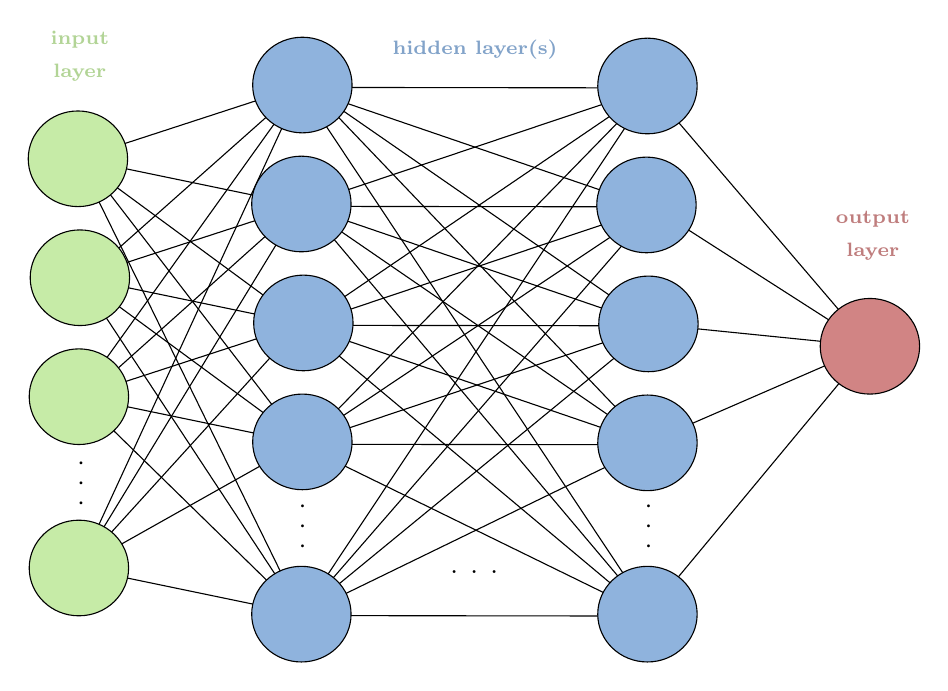
\begin{tikzpicture}[x=0.5pt,y=0.5pt,yscale=-1,xscale=1]
       %uncomment if require: \path (0,496); %set diagram left start at 0, and has height of 496
 
       %Straight Lines [id:da3125603624631026] 
       \draw    (205.85,243.68) -- (456.31,453.44) ;
       %Straight Lines [id:da4017136284587772] 
       \draw    (44.71,124.36) -- (206.2,71.74) ;
       %Straight Lines [id:da2227878135161746] 
       \draw    (46.14,210.32) -- (207.63,157.71) ;
       %Straight Lines [id:da35416891916640736] 
       \draw    (45.42,296.29) -- (206.92,243.68) ;
       %Straight Lines [id:da16193112504220186] 
       \draw    (45.42,420.09) -- (206.2,329.65) ;
       %Straight Lines [id:da3497039034753928] 
       \draw    (44.71,124.36) -- (205.49,157.71) ;
       %Straight Lines [id:da24573604202629373] 
       \draw    (46.14,210.32) -- (206.92,243.68) ;
       %Straight Lines [id:da01718938654762414] 
       \draw    (45.42,296.29) -- (206.2,329.65) ;
       %Straight Lines [id:da4694218304226967] 
       \draw    (45.42,420.09) -- (206.2,453.44) ;
       %Straight Lines [id:da6780505366621903] 
       \draw    (44.71,124.36) -- (206.92,243.68) ;
       %Straight Lines [id:da3700806633588325] 
       \draw    (46.14,210.32) -- (208.35,329.65) ;
       %Straight Lines [id:da7204661169538961] 
       \draw    (45.42,296.29) -- (206.2,453.44) ;
       %Straight Lines [id:da03352111792760715] 
       \draw    (49.89,126.59) -- (206.2,329.65) ;
       %Straight Lines [id:da7880697711535636] 
       \draw    (44.71,124.36) -- (206.2,453.44) ;
       %Straight Lines [id:da8177807044758987] 
       \draw    (46.14,210.32) -- (206.2,453.44) ;
       %Straight Lines [id:da5902292990985858] 
       \draw    (49.89,210.5) -- (206.2,71.74) ;
       %Straight Lines [id:da7293359024356544] 
       \draw    (45.42,296.29) -- (206.2,71.74) ;
       %Straight Lines [id:da8672682409124693] 
       \draw    (45.42,420.09) -- (206.2,71.74) ;
       %Straight Lines [id:da14015258542164877] 
       \draw    (52.03,295.09) -- (205.49,157.71) ;
       %Straight Lines [id:da6510778766409582] 
       \draw    (45.42,420.09) -- (205.49,157.71) ;
       %Straight Lines [id:da19048953930291812] 
       \draw    (45.42,420.09) -- (205.85,243.68) ;
       %Straight Lines [id:da5900414918521127] 
       \draw    (205.52,72.77) -- (459.29,73.12) ;
       %Straight Lines [id:da9923475282888197] 
       \draw    (204.06,158.74) -- (459.29,73.12) ;
       %Straight Lines [id:da6224502087859033] 
       \draw    (206.98,244.71) -- (462.21,159.09) ;
       %Straight Lines [id:da21387151774072322] 
       \draw    (205.52,330.68) -- (460.75,245.05) ;
       %Straight Lines [id:da40912543404428503] 
       \draw    (205.52,454.47) -- (459.29,331.02) ;
       %Straight Lines [id:da6756606943081097] 
       \draw    (208.44,158.74) -- (462.21,159.09) ;
       %Straight Lines [id:da16137493446626694] 
       \draw    (206.98,244.71) -- (460.75,245.05) ;
       %Straight Lines [id:da10150687813127202] 
       \draw    (205.52,330.68) -- (459.29,331.02) ;
       %Straight Lines [id:da0030866090013578207] 
       \draw    (205.52,454.47) -- (459.29,454.82) ;
       %Straight Lines [id:da5047969586038915] 
       \draw    (206.98,244.71) -- (459.29,73.12) ;
       %Straight Lines [id:da16781805884673007] 
       \draw    (204.43,334.29) -- (459.29,73.12) ;
       %Straight Lines [id:da5565130910620758] 
       \draw    (205.52,454.47) -- (459.29,73.12) ;
       %Straight Lines [id:da36371826499194726] 
       \draw    (205.52,454.47) -- (462.21,159.09) ;
       %Straight Lines [id:da11821496918512042] 
       \draw    (205.52,330.68) -- (462.21,159.09) ;
       %Straight Lines [id:da7692636391915034] 
       \draw    (205.52,72.77) -- (457.83,159.09) ;
       %Straight Lines [id:da6770318174394677] 
       \draw    (208.44,158.74) -- (460.75,245.05) ;
       %Straight Lines [id:da9309923147992141] 
       \draw    (206.98,244.71) -- (459.29,331.02) ;
       %Straight Lines [id:da7413198534186101] 
       \draw    (213.18,73.63) -- (460.75,245.05) ;
       %Straight Lines [id:da26068921273410117] 
       \draw    (213.18,73.63) -- (459.29,331.02) ;
       %Straight Lines [id:da8585525579192329] 
       \draw    (205.52,72.77) -- (459.29,454.82) ;
       %Straight Lines [id:da2270863173532055] 
       \draw    (213.18,162.87) -- (459.29,454.82) ;
       %Straight Lines [id:da5864780819119888] 
       \draw    (205.52,330.68) -- (459.29,454.82) ;
       %Straight Lines [id:da16348930210331503] 
       \draw    (205.52,454.47) -- (460.75,245.05) ;
       %Straight Lines [id:da2425074417898001] 
       \draw    (208.44,158.74) -- (459.29,331.02) ;
       %Straight Lines [id:da13422732156968453] 
       \draw    (456.31,71.74) -- (617.09,259.84) ;
       %Straight Lines [id:da7308781194762678] 
       \draw    (457.74,157.71) -- (617.09,259.84) ;
       %Straight Lines [id:da5359704776892366] 
       \draw    (457.02,243.68) -- (617.09,259.84) ;
       %Straight Lines [id:da3406152128273612] 
       \draw    (456.31,329.65) -- (617.09,259.84) ;
       %Straight Lines [id:da14904168253418448] 
       \draw    (456.31,453.44) -- (617.09,259.84) ;
       %Shape: Ellipse [id:dp8560274429988182] 
       \draw  [fill={rgb, 255:red, 198; green, 235; blue, 167 }  ,fill opacity=1 ] (8.8,124.36) .. controls (8.8,105.27) and (24.88,89.8) .. (44.71,89.8) .. controls (64.54,89.8) and (80.62,105.27) .. (80.62,124.36) .. controls (80.62,143.44) and (64.54,158.91) .. (44.71,158.91) .. controls (24.88,158.91) and (8.8,143.44) .. (8.8,124.36) -- cycle ;
       %Shape: Ellipse [id:dp5971121909630736] 
       \draw  [fill={rgb, 255:red, 198; green, 235; blue, 167 }  ,fill opacity=1 ] (10.23,210.32) .. controls (10.23,191.24) and (26.31,175.76) .. (46.14,175.76) .. controls (65.97,175.76) and (82.05,191.24) .. (82.05,210.32) .. controls (82.05,229.41) and (65.97,244.88) .. (46.14,244.88) .. controls (26.31,244.88) and (10.23,229.41) .. (10.23,210.32) -- cycle ;
       %Shape: Ellipse [id:dp024903598729203225] 
       \draw  [fill={rgb, 255:red, 198; green, 235; blue, 167 }  ,fill opacity=1 ] (9.51,296.29) .. controls (9.51,277.21) and (25.59,261.73) .. (45.42,261.73) .. controls (65.25,261.73) and (81.33,277.21) .. (81.33,296.29) .. controls (81.33,315.38) and (65.25,330.85) .. (45.42,330.85) .. controls (25.59,330.85) and (9.51,315.38) .. (9.51,296.29) -- cycle ;
       %Shape: Ellipse [id:dp2752980849146809] 
       \draw  [fill={rgb, 255:red, 198; green, 235; blue, 167 }  ,fill opacity=1 ] (9.51,420.09) .. controls (9.51,401) and (25.59,385.53) .. (45.42,385.53) .. controls (65.25,385.53) and (81.33,401) .. (81.33,420.09) .. controls (81.33,439.17) and (65.25,454.64) .. (45.42,454.64) .. controls (25.59,454.64) and (9.51,439.17) .. (9.51,420.09) -- cycle ;
 
       %Shape: Ellipse [id:dp22212680764969794] 
       \draw  [fill={rgb, 255:red, 143; green, 179; blue, 221 }  ,fill opacity=1 ] (171.01,71.06) .. controls (171.01,51.97) and (187.09,36.5) .. (206.92,36.5) .. controls (226.75,36.5) and (242.83,51.97) .. (242.83,71.06) .. controls (242.83,90.14) and (226.75,105.61) .. (206.92,105.61) .. controls (187.09,105.61) and (171.01,90.14) .. (171.01,71.06) -- cycle ;
       %Shape: Ellipse [id:dp31615925311964466] 
       \draw  [fill={rgb, 255:red, 143; green, 179; blue, 221 }  ,fill opacity=1 ] (170.3,157.02) .. controls (170.3,137.94) and (186.37,122.46) .. (206.2,122.46) .. controls (226.04,122.46) and (242.11,137.94) .. (242.11,157.02) .. controls (242.11,176.11) and (226.04,191.58) .. (206.2,191.58) .. controls (186.37,191.58) and (170.3,176.11) .. (170.3,157.02) -- cycle ;
       %Shape: Ellipse [id:dp763257580789] 
       \draw  [fill={rgb, 255:red, 143; green, 179; blue, 221 }  ,fill opacity=1 ] (171.73,242.99) .. controls (171.73,223.9) and (187.8,208.43) .. (207.63,208.43) .. controls (227.47,208.43) and (243.54,223.9) .. (243.54,242.99) .. controls (243.54,262.08) and (227.47,277.55) .. (207.63,277.55) .. controls (187.8,277.55) and (171.73,262.08) .. (171.73,242.99) -- cycle ;
       %Shape: Ellipse [id:dp41332126656266754] 
       \draw  [fill={rgb, 255:red, 143; green, 179; blue, 221 }  ,fill opacity=1 ] (171.01,328.96) .. controls (171.01,309.87) and (187.09,294.4) .. (206.92,294.4) .. controls (226.75,294.4) and (242.83,309.87) .. (242.83,328.96) .. controls (242.83,348.05) and (226.75,363.52) .. (206.92,363.52) .. controls (187.09,363.52) and (171.01,348.05) .. (171.01,328.96) -- cycle ;
       %Shape: Ellipse [id:dp3269904901419234] 
       \draw  [fill={rgb, 255:red, 143; green, 179; blue, 221 }  ,fill opacity=1 ] (170.3,453.44) .. controls (170.3,434.35) and (186.37,418.88) .. (206.2,418.88) .. controls (226.04,418.88) and (242.11,434.35) .. (242.11,453.44) .. controls (242.11,472.53) and (226.04,488) .. (206.2,488) .. controls (186.37,488) and (170.3,472.53) .. (170.3,453.44) -- cycle ;
       %Shape: Ellipse [id:dp43598218516443177] 
       \draw  [fill={rgb, 255:red, 143; green, 179; blue, 221 }  ,fill opacity=1 ] (420.4,71.74) .. controls (420.4,52.66) and (436.48,37.18) .. (456.31,37.18) .. controls (476.14,37.18) and (492.22,52.66) .. (492.22,71.74) .. controls (492.22,90.83) and (476.14,106.3) .. (456.31,106.3) .. controls (436.48,106.3) and (420.4,90.83) .. (420.4,71.74) -- cycle ;
       %Shape: Ellipse [id:dp5839593265260355] 
       \draw  [fill={rgb, 255:red, 143; green, 179; blue, 221 }  ,fill opacity=1 ] (419.69,157.71) .. controls (419.69,138.62) and (435.76,123.15) .. (455.6,123.15) .. controls (475.43,123.15) and (491.5,138.62) .. (491.5,157.71) .. controls (491.5,176.8) and (475.43,192.27) .. (455.6,192.27) .. controls (435.76,192.27) and (419.69,176.8) .. (419.69,157.71) -- cycle ;
       %Shape: Ellipse [id:dp5046190422661424] 
       \draw  [fill={rgb, 255:red, 143; green, 179; blue, 221 }  ,fill opacity=1 ] (421.12,243.68) .. controls (421.12,224.59) and (437.19,209.12) .. (457.02,209.12) .. controls (476.86,209.12) and (492.93,224.59) .. (492.93,243.68) .. controls (492.93,262.77) and (476.86,278.24) .. (457.02,278.24) .. controls (437.19,278.24) and (421.12,262.77) .. (421.12,243.68) -- cycle ;
       %Shape: Ellipse [id:dp04717464708306185] 
       \draw  [fill={rgb, 255:red, 143; green, 179; blue, 221 }  ,fill opacity=1 ] (420.4,329.65) .. controls (420.4,310.56) and (436.48,295.09) .. (456.31,295.09) .. controls (476.14,295.09) and (492.22,310.56) .. (492.22,329.65) .. controls (492.22,348.73) and (476.14,364.21) .. (456.31,364.21) .. controls (436.48,364.21) and (420.4,348.73) .. (420.4,329.65) -- cycle ;
       %Shape: Ellipse [id:dp9408343992389916] 
       \draw  [fill={rgb, 255:red, 143; green, 179; blue, 221 }  ,fill opacity=1 ] (420.4,453.44) .. controls (420.4,434.35) and (436.48,418.88) .. (456.31,418.88) .. controls (476.14,418.88) and (492.22,434.35) .. (492.22,453.44) .. controls (492.22,472.53) and (476.14,488) .. (456.31,488) .. controls (436.48,488) and (420.4,472.53) .. (420.4,453.44) -- cycle ;
       %Shape: Ellipse [id:dp47294074537144504] 
       \draw  [fill={rgb, 255:red, 209; green, 132; blue, 132 }  ,fill opacity=1 ] (581.18,259.84) .. controls (581.18,240.75) and (597.26,225.28) .. (617.09,225.28) .. controls (636.92,225.28) and (653,240.75) .. (653,259.84) .. controls (653,278.93) and (636.92,294.4) .. (617.09,294.4) .. controls (597.26,294.4) and (581.18,278.93) .. (581.18,259.84) -- cycle ;
       % Text Node
       \draw (50,340) node [anchor=north west][inner sep=0.75pt]  [rotate=-90] [align=left] {. . .};
       % Text Node
       \draw (210,371) node [anchor=north west][inner sep=0.75pt]  [rotate=-90] [align=left] {. . .};
       % Text Node
       \draw (460,371) node [anchor=north west][inner sep=0.75pt]  [rotate=-90] [align=left] {. . .};
       % Text Node
       \draw (312,420) node [anchor=north west][inner sep=0.75pt]  [rotate=0] [align=left] {. . .};
       % Text Node
       \draw (22,30) node [anchor=north west][inner sep=0.75pt]  [color={rgb, 255:red, 198; green, 235; blue, 167 }  ,opacity=1 ] [align=left] {\begin{minipage}[lt]{22.16pt}\setlength\topsep{0pt}
       \begin{center}
       {\scriptsize \textcolor[rgb]{0.7,0.83,0.59}{\textbf{input\\layer}}}
       \end{center}
 
       \end{minipage}};
       % Text Node
       \draw (270.19,36.82) node [anchor=north west][inner sep=0.75pt]   [align=left] {{\scriptsize \textcolor[rgb]{0.51,0.64,0.79}{\textbf{hidden layer(s)}}}};
       % Text Node
       \draw (590.42,160.07) node [anchor=north west][inner sep=0.75pt]   [align=left] {\begin{minipage}[lt]{26.92pt}\setlength\topsep{0pt}
       \begin{center}
       {\scriptsize \textbf{\textcolor[rgb]{0.75,0.49,0.49}{output\\layer}}}
       \end{center}
 
       \end{minipage}};
       % Text Node
    %    \draw (80.17,460) node [anchor=north west][inner sep=0.75pt]   [align=left] {{\tiny f(x) = ReLu}};
       % Text Node
    %    \draw (295.11,460) node [anchor=north west][inner sep=0.75pt]   [align=left] {{\tiny f(x) = ReLu}};
       % Text Node
    %    \draw (528.6,460) node [anchor=north west][inner sep=0.75pt]   [align=left] {{\tiny f(x) = Sigmoid}};
 
 
    \end{tikzpicture}
    \caption[Basic Neural Network Illustration]{Basic illustration of a network with two hidden layers.}
    \label{fig:FFN}
\end{figure}


\subsection{Back Propagation algorithm}
So far we have only explained Feed Forward networks, which helps us to compute the output of the NN in term of basic linear algebra. We mentioned the possibility to adjust the weight and biases, but never explained how. 
Now is the time to dive into that subject, as we will explain the back propagation algorithm. What we want to know is how the changes in the biases and weights in the network change the cost function, and how we could use the final 
output to modify the weights? Before we derive these equations we start by a plain regression problem, using the Mean Squared Error (MSE) as a cost function for pedagogical reasons
\begin{equation}\label{eq:cost}
    C(\hat{W})=\frac{1}{2}\sum_{i=1}^n(y_i-t_i)^2
\end{equation}
where $\hat{W}$ is the matrix containing all the weights and (more importantly) $t_i$ are the targets, which are the labels of events telling whether we have a signal or background event. To generalise this we 
first have to generalise to Eq. (\ref{eq:weightedsum}) for a layer $l$
$$
    z_i^l=\sum_{j=1}^Mw^l_{ij}y^{l-1}_j + b^l_i \Leftrightarrow \hat{z}^l=\left(\hat{W}^l\right)^T\hat{y}^{l-1} + \hat{b}^l
$$
where the right side is written in matrix notation. From the definition of $z_j^l$ with an activation function, Eq. (\ref{eq:activation}), we have
\begin{equation}\label{eq:partzw}
    \frac{\partial z_j^l}{\partial w_{ij}^l} = y_i^{l-1}
\end{equation}
and
$$
\frac{\partial z_j^l}{\partial y_i^{l-1}} = w_{ij}^l
$$
which again, with the definition of the sigmoid activation function, Eq. (\ref{eq:sig}), gives us
\begin{equation}\label{eq:partyz}
    \frac{\partial y^l_j}{\partial z_j^{l}} = y_j^l(1-y_j^l)=f(z_j^l)(1-f(z_j^l))
\end{equation}
Furthermore, we need to take the derivative of Eq. (\ref{eq:cost}) with respect to the weights, doing so for a respective layer $l=L$ we have
$$
    \frac{\partial C(\hat W ^L) }{\partial w_{jk}^L}=\left(y_j^L-t_j\right)\frac{\partial y_j^L}{\partial w_{jk}^L}
$$
where the last partial derivative is easily computed using the chain rule with Eq. (\ref{eq:partzw}) and Eq. (\ref{eq:partyz})
$$
\frac{\partial y_j^L}{\partial w_{jk}^L} = \frac{\partial y^L_j}{\partial z_j^{L}}\frac{\partial z_j^l}{\partial w_{jk}^L} = y_j^L(1-y_j^L)y_k^{L-1}
$$
Such that
\begin{equation}\label{eq:CostW}
    \frac{\partial C(\hat W ^L) }{\partial w_{jk}^L}=\left(y_j^L-t_j\right)y_j^L(1-y_j^L)y_k^{L-1} :=\delta_j^Ly_k^{L-1}
\end{equation}
where we have defined the error
\begin{equation}\label{eq:delta}
    \delta_j^L:=\left(y_j^L-t_j\right)y_j^L(1-y_j^L)=f'(z_j^L)\frac{\partial C}{\partial y_j^L} 
\end{equation}
or in matrix form
$$
\delta^L = f'(\hat z ^L)\circ \frac{\partial C}{\partial \hat y ^L}
$$
where on the right hand side we wrote this as a Hadamard product\footnote{Also called \textit{element-wise} product, $(A\circ B)_{ij} = (A\odot B)_{ij} = (A)_{ij}(B)_{ij}$}. This error $\delta^L$ is an important expression, since as we can see in the index form of this expression in Eq. (\ref{eq:delta}), we can measure how fast 
the cost function is changing as a function of the $j$-th output activation. This means that if the cost function doesn't depend on a particular neuron $j$, then $\delta_j^L$ would be small.  \\
\\We also notice that everything in Eq. (\ref{eq:delta}) is easily computed. Thus we can also see how the weight changes the cost function using Eq. (\ref{eq:CostW}) quite easily. 
Another thing we can compute with Eq. (\ref{eq:delta}) is
$$
\delta_j^L=\frac{\partial C}{\partial z_j^L} =\frac{\partial C}{\partial y_j^L}\frac{\partial y_j^L}{\partial z_j^L}
$$
which can be interpreted in terms of the biases $b_j^L$ as
\begin{equation}\label{eq:bias}
    \delta_j^L=\frac{\partial C}{\partial b_j^L}\frac{\partial b_j^L}{\partial z_j^L} = \frac{\partial C}{\partial b_j^L} 
\end{equation}
where the error $\delta_j^L$ is exactly equal to the rate of change of the cost function as a function of the bias.\\
\\Something interesting is that when using Eq. (\ref{eq:CostW} - \ref{eq:bias}) we see that if a neuron output $y_j^L$ is small, then the gradient term, Eq. (\ref{eq:CostW}), will also be small. We say then that the weight learns 
slowly, meaning that the contribution of said neuron is less important "to fix" than those that have a higher weight. Of course this example is a very simple one to wrap our heads around, but the magic comes when the algorithm is 
evaluating a random neuron in a layer $n$, after using many layers the NN becomes a \textbf{black box} for us to wrap our heads around!\\
\\It is also worth noting that when the activation function is flat at some specific values (which also varies with the chosen function!) the derivative will tend towards zero, making the gradient small, 
meaning the network is learning slow as well. To finish up our back propagation algorithm we still need one equation. We are now going to propagate backwards in order to determine the weights and biases. 
We start by representing the error in the layer before the final one $L-1$ in term of the errors of the output layer. If we try to express Eq. (\ref{eq:delta}) in terms of the output layer $l+1$, 
using the chain rule and summing over all $k$ entries we get
$$
\delta_j^l=\sum_k\frac{\partial C}{\partial z_k^{l+1}}\frac{\partial z_k^{l+1}}{\partial z_j^l} =\sum_k \delta_k^{l+1}\frac{\partial z_k^{l+1}}{\partial z_j^l}
$$
recalling Eq. (\ref{eq:weightedsum}) (replacing $1$ with $l+1$) we get
\begin{equation}\label{eq:backprop}
    \delta_j^l=\sum_k\delta_k^{l+1}w_{kj}^{l+1}f'(z_j^l)
\end{equation}
Which is the final equation we needed to start back propagating. 

\subsection{Summary}
To summarize the whole process of the NN
\begin{itemize}
    \item First take the input data $\mathbf{x}$ and the activation $\mathbf{z}_1$ of the input later, and then compute the activation function $f(z)$ to get the next neuron outputs $\mathbf{y}^1$. 
    Mathematically this is taking the first step of the feed forward algorithm, i.e. choosing $l=0$ in Eq. (\ref{eq:MLP})
    \item Secondly we commit all the way in Eq. (\ref{eq:MLP}) and compute all $\mathbf{z}_l$, activation function and $\mathbf{y}^l$.
    \item After that we compute the output error $\bm{\delta}^L$ by using Eq. (\ref{eq:delta}) for all values $j$.
    \item Then we back propagate the error for each $l=L-1,L-2,\cdots,2$ with Eq. (\ref{eq:backprop}).
    \item The last step is then to update the weights and biases using Eq. (\ref{eq:GD}) for each $l$ and updating using
    $$
    w_{jk}^l\leftarrow w_{jk}^l-\eta\delta_j^ly_k^{l-1}
    $$
    and
    $$
    b_j^l \leftarrow b_j^l-\eta\delta_j^l
    $$
\end{itemize}
This whole procedure is usually called an epoch, which we can repeat as many times as we want to better reduce the cost function in hope of converging to the global minima.

\clearpage




\section{Boosted Decision Trees}
In the previous chapter, we explored how NNs can aid in the task of signal and background classiciation, such as the one in this thesis where we are looking DM signal in the SM background. In this chapter, we will delve into Boosted Decision Trees (BDTs), 
another powerful tool for binary classifications. BDTs, unlike neural networks, are not based on simulating biological neurons. Instead, they rely on decision trees, a simple yet powerful idea that has been around for decades. \cite{Morgan1963ProblemsIT, ID3_BDT} 
Decision trees are built by recursively splitting data based on the values of features until a stopping condition is met. BDTs take this idea one step further by training an ensemble of decision trees, where each tree attempts to correct the mistakes of its predecessors.\\
\\BDTs have several advantages over other machine learning algorithms, such as neural networks, for binary classification problems. They are highly interpretable, which allows us to understand how they arrived at their decisions. This is particularly important in this field, 
high energy particle physics, where the ability to interpret results is crucial. BDTs are also highly resilient to overfitting and can handle missing data effectively. Given their strengths, BDTs have been widely used in particle physics for binary classification tasks, 
such as distinguishing signal from background events. The idea of the BDTs used in high energy physics today was proposed as early as 2001 by Friedmann in the paper \textit{Greedy Function Approximation} \cite{BDT_Friedman}, and since then have become an indispensable tool in the field. 
In particular, in the ATLAS collaboration challenge \textit{The Higgs boson machine learning challenge} \cite{HiggsChallenge} the creation of a BDT package called \verb|XGBoost| \cite{XGBoost} increased the popularity even more as they won the challenge. 
Today \verb|XGBoost| has become a standard ML tool used in the field.\\
\\In this chapter, we will explore the theory behind BDTs in the context of \textit{extreme gradient boosting}, for this we we are mainly interested in two ways of making DTs, a set of Classification And Regression Trees (CART). 
The theory is mainly based of Hjort-Jensens lecture notes \cite{MORTYY4, MORTYY5} and section 2 on the original \verb|XGBoost| paper \cite{XGBoost}.
\newpage
\subsection{Decision trees}
Starting with Decision Trees (DT) in the context of this DM search. The idea behind DTs is to find the most important features which contain the most information of signal (DM), and then split the dataset along the values of these features with the goal of creating a dataset containing pure signal. 
As we are going to use kinematical variables as features we will use this to both augment and automate the classical cut and count method (Chapter \ref{sec:data_anal}), which is based of making kinematical cuts on the variables. To find which kinematical features are most important 
in splitting the dataset we have to achieve a stopping criteria where we end up on a so-called \textit{leaf node}.\\
\\A DT is typically divided into a \textit{root nodes}, \textit{interior nodes} and a final \textit{leaf nodes}, also called leaves, which are all connected by \textit{branches}, hence the name decision \textit{tree}. As mentioned in the start of this chapter, we will look at two ways of making DTs, 
the first one we will look at is the \textit{regression tree}. 

\subsection{Regression trees}
As previously mentioned the leaves contain the prediction of a trained network, and are used to make new predictions on new datasets based on the information the DT learning in the branching process. As how to construct trees, there are mainly two steps we need to follow:
\begin{enumerate}
    \item Split the predictior space (set of possible values $x_1,x_2,\cdots,x_p$) into $J$ distinct and non-overlapping regions, $R_1,R_2,\cdots,R_J$\todo{is this too similar to 9.3 in \cite{MORTYY4}?}
    \item For every observation that fals into the region $R_j$, we make the same prediction, which is the mean of the response values for the training observations in $R_J$
\end{enumerate}
But how do we construct the regions $R_1,R_2,\cdots,R_J$? In theory these regions could have any shape, but for simplicity and pedagogial reasons we will choose to divide the predictor shpe into high-dimensional rectangles, or boxes. This means that the goal is to find boxes 
$R_1,R_2,\cdots,R_J$ that minimize a \textit{cost function}, which again, for pedagogical reasons will be the a MSE (Eq. (\ref{eq:cost})), defined as 
$$
\sum_{j=1}^{J}\sum_{i\in R_j}(y_i -\bar{y}_{R_j})^2
$$
where $\bar{y}_{R_j}$ is the mean response for the training observations withing box $j$. Ideally we would consider every possible partition of the feature space into $J$ boxes, but his is computationally infeasable. Thus the common apporach is to begin at the top of the tree, 
where all observations belong to a single region, and then split the predictor space; where every split is indicated via two new branches down in the tree. This is greedy (as in \textit{Greedy Function Approximation} \cite{BDT_Friedman}) since the best split is mad in the first step, 
rather than looking ahead and picking a split that might lead to a better tree in a future step.\\ 
To make any split we start by selecting the predictor $x_j$ and a cutpoint $s$ that splits the predictor space into two regions $R_1$ and $R_2$
$$
\{X\vert x_j < s\} \quad\text{and}\quad \{X\vert x_j \ge s\}
$$
so that we obtain the lowest MSE, 
$$
\sum_{i:x_i\in R_1}(y_i-\bar{y}_{R_1})^2 + \sum_{i:x_i\in R_2}(y_i-\bar{y}_{R_2})^2
$$
where we consider all predictors $x_1,x_2,\cdots,x_p$ and each possible value $s$ for each of them, where these values can be randomly assigned numbers. For any $j$ and $s$ we define the pair of half-planes where $\bar{y}_{R_1}$ and $\bar{y}_{R_2}$ are the mean responses for the training 
observations in $R_1(j,s)$ and $R_2(j,s)$ respectively. The goal is to find the value $j$ and $s$ such that we minimize the cost function, which can be done quickly depending on the number of predictors.\\
\\Then we repeat the process looking for the best predictor and best cutpoint, but instead of stopping with two regions, we split one of the two into another two regions creating a total of three regions. This is called the depth of a tree, and we can in principle continue to split indefinetely, 
however one usually sets a stopping criterion on how many events should be at a leaf.\\
\\The method explored above is straight forward, but often leads to overfitting and unnecessarily large and complicated trees. To mediate this one usually uses a so-called \textit{Cost complexity} pruning algorithm. 
For regression precedures, the algorithm, rather than considering every possible subtree, comnsiders a sequence of trees indexed by a nonnegative tuning parameter $\alpha$. For each value of this $\alpha$ there corresponds a subtree $T\in T_0$ such that
\begin{equation}\label{eq:REG_tree_Cost}
    \sum_{m=1}^{\bar{T}}\sum_{i:x_i\in R_m}(y_i -\bar{y}_{R_m})^2 + \alpha T
\end{equation}
is as small possible. In the equation above $T$ is the number of terminal nodes of the tree $T$, $R_m$ is the rectangle corrresponding to the $m$-th terminal node. This tuning parameter $\alpha$ controls a trade-off between the subtree's complexity and its fit to the training data. 
As $\alpha$ increases, the above equation will give us a higher value, meaning that our trees would normally prioritize less complex models. This precedure is repeated untill we minimize Eq. (\ref{eq:REG_tree_Cost}) and choose a suitable value for $\alpha$. This is the essense of regression trees.

\subsection{Classification trees}
The second DT type we will study is the \textit{classification tree}. Classification trees are very similar to regresion trees, except that they are used to predict a qualitative response rather than a quantitative one. This means that classification trees are used for predictive modeling in 
which the output variable is discrete, such as classifying an email as spam or not spam, or predicting whether an event in our dataset is a DM signal or SM background event.\\
\\Like regression trees, classification trees recursively split the data based on the values of input variables until a stopping condition is met. However, the splitting criteria for classification trees are different. Classification trees cannot use the MSE function used in regression trees 
as a criterion for making binary splits, instead they use the \textit{classification error rate}. The classification error rate, classification trees have discrete outputs, is simply the fraction of the training observations in a region that do not belong to the most common class.\\
\\Classification trees use measures such as Gini index or the entropy to determine quality of a split at each node. The idea behind these quality measures is to select the split that maximizes the separation between the different categories of the output variable.\\
\\If a classification tasks takes for example $k=1,2,\cdots,K$ values as outputs, we can define a probability distribution function $p_{mk}$ that represents the number of observations of $k$ in a region $R_m$ with $N_m$ observations. We can represent this likelihood function in terms 
of the proportion $I(y_i=k)$ of obervations of this output in region $R_m$ as
$$
p_{mk}=\frac{1}{N_m}\sum_{x_i\in R_m}I(y_i=k)
$$
where $p_{mk}$ represents the majority class of observations in region $m$. The tree most common ways of splitting a node are given by: The misclassification error
$$
p_{mk}=\frac{1}{N_m}\sum_{x_i\in R_m}I(y_i\ne k) = 1-p_{mk}
$$
The Gini index $G$
\begin{equation}\label{eq:gini}
    G=\sum_{k=1}^K p_{mk}(1-p_{mk})
\end{equation}
and the entropy $s$
$$
s=-\sum_{k=1}^K p_{mk}\log(p_{mk})
$$

\subsection{The CART algorithm} 
As we are going to look at extreme gradient boosting, the main algorithm for this type of DT is the Classification And Regression Tree (CART). For classification, the CART algorithm splits the dataset in two subsetsusing a single feature $k$ and treshold $t_k$. This could for example be 
a treshhold set by a value of the invariant mass of an event we are trying to classify as background or signal. The way we optimize the pair $(k,t_k)$ such that we get the purest subset is by for example using the gini factor $G$. With this the cost function tries to minimize
$$
C(k,t_k)=\frac{m_{left}}{m}G_{left}+\frac{m_{right}}{m}G_{right}
$$
where $G_{left/right}$ calculats the impurity of the left/right subset using Eq. (\ref{eq:gini}) and $m_{left/right}$ is the number of events in the left/right subset. Once the algorithm successfully splits the training set into two, it splits the subsets using the same agorithm, and so on, 
recursively. For our purposes we will make the DT stop searching for the pair $(k,t_k)$ once we have reaches the maximum depht we chose, or whenever the sum of the weights on a leaf is one. Both of these are hyperparameters that need to be optimized, for that see Chapter \ref{sec:BDTGriddy}.\\
\\The CART algorithm for regression works similarly to the one for classification, but instead of trying to split the training set in a way that minimizes the gini or entropy impurity, it tries to split the training set in a way that minimizes the (MSE). Meaning that we have
$$
C(k,t_k)=\frac{m_{left}}{m}MSE_{left}+\frac{m_{right}}{m}MSE_{right}
$$
with
$$
MSE_{node} = \frac{1}{m_{node}}\sum_{i\in node}(\bar{y}_{node} -y_i)^2
$$
and
$$
\bar{y}_{node} = \frac{1}{m_{node}}\sum_{i\in node}y_i
$$

\subsection{Ensemble modeling and (extreme) gradient boosting}
Now that we have explained how DTs wor, we still need more information to get the full picute of \textit{Boosted} DTs. For this section of the chapter we. As we are going to look at a massive dataset, a single tree is not strong enough to be used in practice. What is actually used is the \textit{ensemble model}, which 
sums up the prediction of multiple trees togheter. What is important of this models is that the different trees we are summing togheter try to complement each other. For example if the first split on one tree is on the invariant mass of a dilepton pair, while on another tree it is the MET, 
then we know physically that these are important features that DM + dilepton models have as a signature, meaning that it should be a good combination. Mathematically, we can write the prediction of an ensemble model in the form
\begin{equation}\label{eq:ensemble}
    \hat{y}_i =\sum_{k=1}^{K}f_k(x_i),\quad f_k\in\mathcal{F}
\end{equation}
where $K$ is the number of trees we want to sum over, $f_k$ is a function of the functional space $\mathcal{F}$, where $\mathcal{F}$ is the set of all possible CARTs. With this we want to minime a the objective function of the form
$$
    \mathcal{L} = \sum_{i}^{n}C(y_i,\hat{y}_i)+\sum_{k=1}^{K}\Omega(f_k)
$$
where we sum over $n$ leaves, $C$ is training cost function (for example it can be the MSE), and $\Omega(f_k)$ is the complexity of the tree $f_k$, which penalizes the more complex models. We can see from both functions above that we need to learn all trees at once to make predictions, this is however both 
computationally demanding and intractable. Instead, we can use an additive strategy, where we fix what we have learned, and add a new tree at a time. Using Eq. \ref{eq:ensemble} with 0 trees and going up we see that we get
\begin{align*}
    &\hat{y}_i^{(0)} = 0\\
    &\hat{y}_i^{(1)} = f_1(x_i)=\hat{y}_i^{(0)}+f_1(x_i)\\
    &\hat{y}_i^{(2)} = f_1(x_i)+f_2(x_i)=\hat{y}_i^{(1)}+f_2(x_i)\\
    &\hat{y}_i^{(3)} = f_1(x_i)+f_2(x_i)+f_3(x_i)=\hat{y}_i^{(2)}+f_3(x_i)
\end{align*}
and so on. Mathematically we see that a prediction at step $t$ as in $\hat{y}_i^{(t)}$ takes the form
\begin{equation}\label{eq:eff_ensemble}
    \hat{y}_i^{(t)}=\sum_{k=1}^{t}f_k(x_i) = \hat{y}_i^{(t-1)}+f_t(x_i)
\end{equation}
Such that we can now write the objective to be
\begin{equation}
    \mathcal{L}^{(t)}=\sum_{i}^{n}C(y_i,\hat{y}_i^{(t-1)}+f_t(x_i))+\Omega(f_t)
\end{equation}
from which we can set up our choice for cost function. In general case we take the Taylor expansion of the loss function up to the second order such that we get
$$
    \mathcal{L}^{(t)}=\sum_{i}^{n}\left[C(y_i,\hat{y}_i^{(t-1)})+g_i f_t(x_i)+\frac{1}{2}h_i f_t^2(x_i)\right]+\Omega(f_t)+const
$$
where 
$$
    g_i \equiv \partial_{\hat{y}_i^{(t-1)}}C(y_i,\hat{y}_i^{(t-1)}) \quad\text{and}\quad   h_i \equiv \partial^2_{\hat{y}_i^{(t-1)}}C(y_i,\hat{y}_i^{(t-1)})
$$
Such that the specific objective at step $t$ becomes
\begin{equation}\label{eq:new_obj}
    \sum_{i=1}^{n}\left[ g_i f_t(x_i) +\frac{1}{2}h_i f_t^2(x_i)\right] +\Omega(f_t)
\end{equation}
where we removed all constants. Such that Eq (\ref{eq:new_obj}) becomes the optimization goal for the new tree. As we can see the above equation can take into account any cost function as it is written in a general form with a Taylor expansion. Furthermore, we can rewrite this by expanding 
$$
\Omega(f_t) \rightarrow \alpha T + \frac{1}{2}\lambda\sum_{j=1}^{T} w_j^2 
$$ 
where the first term is the same as in Eq. (\ref{eq:REG_tree_Cost}), and the second is called the \textit{regularization term} (see Chapter \ref{sec:cost_func}). Inserting this into Eq. (\ref{eq:new_obj}) we get
$$
\mathcal{L}^{(t)} = \sum_{j=1}^{T}\left[\left(\sum_{i=1}^{n} g_i\right)w_j +\frac{1}{2}\left(\sum_{i=1}^{n} h_i +\lambda \right)w_j^2\right] +\alpha T
$$
such that with a fixed tree structure, $q$, we can define the optimal weight $w_j^*$ on a leaf $j$ as 
\begin{equation}\label{eq:opt_wgt_bdt}
    w_j^*=-\frac{\sum_{i=1}^{n} g_i}{\sum_{i=1}^{n} h_i+\lambda}
\end{equation}
and correspondingly the optimal objective reduction
\begin{equation}\label{eq:opt_obj_bdt}
    \mathcal{L}^{(t)}(q)=-\frac{1}{2}\sum_{j=1}^{T}\frac{(\sum_{i=1}^{n} g_i)^2}{\sum_{i=1}^{n} h_i+\lambda}+\alpha T
\end{equation}
With both of these equations we have all we need to use BDTs, the extreme part of the gradient boosting is something the \verb|XGBoost| algorithm has implemented in terms of system optimization, such as parallelising the tree boosting task, and can be read in more detail on section 4 of the original paper \cite{XGBoost}.


\subsection{Summary}
So in short BDTs split datasets based on different values of the features on the dataset, figure \ref{fig:DT_ilus} shows an illustration of how DTs work.
\graphicspath{{../../figures/}}
\begin{figure}[!ht]
	\centering
    \includegraphics[width=1\textwidth]{BDT_image.png}
    \caption[Basic Decision Tree illustration]{Image showcasing how decision trees work by splitting a dataset of $N$ events with $M$ features whenever a treshhold $X, Y$ or $Z$ for a feature is passed. The label $S$ and $B$ state whether the event is signal or background respectively.}\label{fig:DT_ilus}
\end{figure}
\\The above illustration just shows how one tree might work, in reality we can choose to have an arbitraty number of trees and combine their results with the ensembling and boosting method. Then after combining the generated tree structures we use Eq. (\ref{eq:opt_wgt_bdt}) and Eq. (\ref{eq:opt_obj_bdt}) 
to minimize the objective to get the most accurate predictions as possible. 

\clearpage
\section{Tools and evaluation methods used for both algorithms}\label{sec:tools}
Now that we have explained how both NNs and BDTs work, we will present the tools and evaluating method that we will use in this thesis. 

\subsection{Cost functions}\label{sec:cost_func}
Cost functions have been mentioned throughout this chapter, but what are they? Cost functions are what we will utilize to evaluate how well the output of the network fares against the target, i.e. if our network "guesses" right whether an event is signal or background, 
thus making this a very important part of our network! Before getting into this we first have to look at logistic regression. Since we are studing a binary classification task where the output is either $t_i=0$ or $t_i = 1$, meaning background or signal. 
We can introduce a polynomial model of order $n$ as
$$
\hat{y}_i=\beta_0+\beta_1x_i+\beta_2x_i^2+\cdots+\beta_nx_i^n
$$
where the hat notation, $\hat y$, symbolises a condensed matrix form of the output of a layer. We can define the probabilities of getting $t_i=0$ or 1 given our input $x_i$ and $\bm{\beta}$ with the help of a logistic function. 
Using this we get the probability as
$$
p(t_i=1\vert x_i,\bm{\beta})=\frac{1}{1+e^{-t_i}}
$$
and
$$
p(t_i=0\vert x_i,\bm{\beta})=1- p(t_i=1\vert x_i,\bm{\beta})
$$
We want to then define the total likelihood for all possible outcomes from a dataset $\mathcal{D}=\{(t_i,x_i)\}$, with the binary labels $t_i\in\{0,1\}$, applying the Maximum Likelihood Estimation (MLE) principle. 
This gives us
$$
P(\mathcal{D}\vert\bm{\beta})=\prod_{i=1}^n\left[p(t_i=1\vert x_i,\bm{\beta})\right]^{t_i}\left[1-p(t_i=1\vert x_i,\bm{\beta})\right]^{1-t_i}
$$
from which we obtain the log-likelihood
$$
C(\bm{\beta})=\sum_{i=1}^n\left(t_i\log p(t_i=1\vert x_i,\bm{\beta})+(1-t_i)\log[1-p(t_i=1\vert x_i,\bm{\beta})]\right)
$$
By taking the parameter $\bm{\beta}$ to first order in $x_i$ and reordering the logarithm we get
\begin{equation}\label{eq:CrossEntropy}
    C(\bm{\beta})=-\sum_{i=1}^n(y_i(\beta_0+\beta_1x_i)-\log(1+\exp(\beta_0+\beta_1x_i)))
\end{equation}
This equation we will use throughtout the thesis and is known as the \textit{cross entropy}. The two beta parameters used are the weight and biases, $\beta_1 = w$ and $\beta_0 = b$. The goal is to change these parameters such that it minimizes the cost function. 
\subsubsection*{L2-regularization}
Furthermore we will add an extra term to the cost function, proportional to the size of the weights. We do this to constrain the size of the weights, so they don't grow out of control, 
this is to reduce \textit{overfitting}. We will use the so-called \textit{L2-norm} \todo{add source for article?}where the cost function becomes
\begin{equation}\label{eq:L2-reg}
    C(\bm\beta)\rightarrow C(\bm\beta)+\lambda\sum_{ij}w_{ij}^2
\end{equation}
meaning that we add a term where we sum up \textbf{all} the weights squared. The factor $\lambda$ is called the regularization parameter. The L2-norm combats overfitting by forcing the weights to be small, but not making them exactly zero. 
This is so that less significant features still have some influence over the final prediction, although small.


\subsection{Sample weight}\label{sec:sample_weight}
A "sample weights" array is an array of numbers that specify how much weight each sample in a batch should have in computing the total loss. 
It is commonly used in imbalanced classification problems (the idea being to give more weight to rarely-seen classes). Taken from the original documentation \cite{tf_sample_wgt}. To mathematically illustrate how this 
weight works is by multiplying a constant term $\chi$ into the cost/loss function that is used further on the error propagation. As an example we can extend the simple MSE, Eq. (\ref{eq:cost}) to
\begin{equation}\label{eq:sample_weight}
    C(\hat{W})=\frac{1}{2}\sum_{i=1}^n\chi_i(y_i-t_i)^2
\end{equation}
This will become an important feature when discussing network optimization in Chapter \ref{chap:ML}, and especially for particle physists as we want to re-weight Monte Carlo events to expected events to correctly showcase kinematical distributions.


\subsection{Area under the ROC-curve}
To evaluate how well our networks do. We will use the acuracy, which literally tells us how many events it guessed right. But also take into account a more advanced metrics, this is the Area Under the "Receiver Operating Characteristic (ROC)" Curve (AUC). 
Before explaining what the AUC is we first need to expclote the ROC curves. The ROC curves helps us illustrate how successfull a network is a \textit{binary classification} (only). The ROC curve, as the name states is a curve, where we plot the \textit{True Positive Rate} (TPR) against 
the \textit{False Positive Rate} (FPR). The TPR is defined by dividing the \textit{True Positive} (TP), which is when the netowrk correctly guesses a signal event to be a signal event, by the \textit{Positive} (P), which is the total number of signal events in the data. 
$$
\text{TPR} =\frac{\text{TP}}{\text{P}}
$$
On the other hand, the FPR is when we divide the \textit{False Positive} (FP), when the network guesses a background event to be signal event, divided by the \textit{Negatives} (N), the total number of background events in the data.
$$
\text{FPR} =\frac{\text{FP}}{\text{N}}
$$
To get a numerical value of how well a network classifies data we thus calculate the AUC. The TP and the FP are both going to be predictions from the networks, which for this thesis will gave an event a score from 0 to 1\footnote{Where 0 means that the network believes an event has 0\% chance of being a signal event, and 1 means that the networks believes with 100\% certainty that an event is a signal event.}, 
meaning that if we had a perfect network which guesses everything correctly we would only get TPs and thus an AUC of 1. If we were to get an area of 0.5 this would mean that the network is randomly guessing whether an event is a signal or background, practically making a coin toss for every event. 
The goal is to have a network to give an AUC score as closely to 1 as possible. \\
\\While only using the accuracy as a metric is not a bad start, it is not favorable to use as a metric if datasets are ubalanced. As en example, if we had a dataset with 100 events, where 95 were background events and 5 were signal events, if we only used accuracy as a metric we would 
be inlcined to think that an accuracy of 95\% is great. However, as the dataset is unbalanced, the network could easily take a shortcut and guess every event to be a background event. Meaning that the network learned nothing.
This is where the AUC comes into play, as this metric highlights whenever a network guesses wrongly in a binary classification. Meaning that if we used the worst case scenario with 95\% accuracy when guessing everything to be background, we would have a TPR = 0 and a FPR = 0, 
if we were to plot this we would get a flat line on the FPR and TPR axis, meaning that it would give us an AUC of 0.5. Highlighting that our network is randomly guessing, and that it needs to be optimized further. In Figure \ref{fig:ROC} we see an example of a ROC curve.
\graphicspath{{../../../Plots/Plot_types/}}
\begin{figure}[!ht]
	\centering
    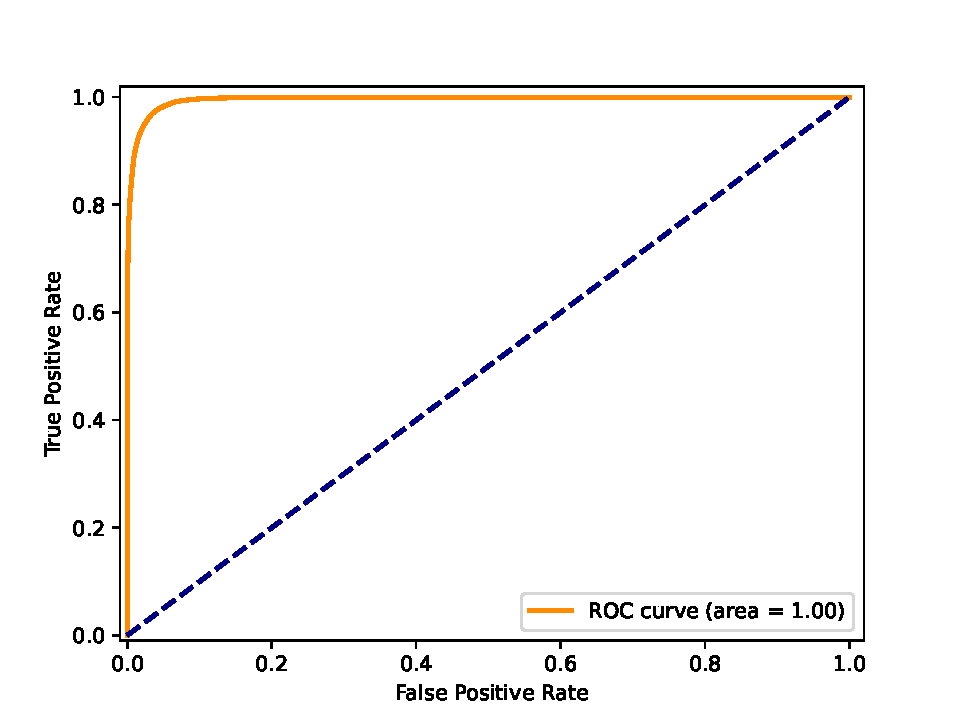
\includegraphics[width=0.65\textwidth]{ROC.pdf}
    \caption[ROC curve illustration]{Illustration of a ROC curve. The orange line is the result of a network, while the dashed blue line is to illustrate a random guess}\label{fig:ROC}
\end{figure}
\\\textit{Comment for farid/eirik, I used wikipedia as a source on the theory here, how do I cite that?}

\subsection{Validation plots}\label{sec:validation}
Another tool that we will use to evaluate how well a network does is by making so-called \textit{validation plots}\todo{Is this the real name of the plots?}. The way these plots work is by first dividing the \textit{already predicted} data set into background and signal. Then making histograms from 0-1 
with the prediction score of the network for each event. As a score closer to 1 means that the network predicts an event to be a signal event, and 0 means that the network predicts a background event. Then we would ideally have all the signal events shoved to the right and all the background events shoved to the left. 
Usually this is not the case in high energy particle physics, as some background events might be similar to signal events. We will therefore utilize this kind of plots to see the ditribution of the network predictions. \\
\\In adition to just sorting events by the ML score, we will also re-weight the events (which are MC events) into expected events\footnote{See Chapter \ref{sec:wgts} for more information}. The difference this makes can be seen in Figure \ref{fig:VAL}. We can however still use the non-re-weighted plots to see how well the network has learned to sort, but these plots will not be 
used in this thesis, and can rather be found on the Github repo. \\
\begin{figure}[!ht]
	\centering
    \begin{subfigure}[b]{0.7\textwidth}
        \centering
        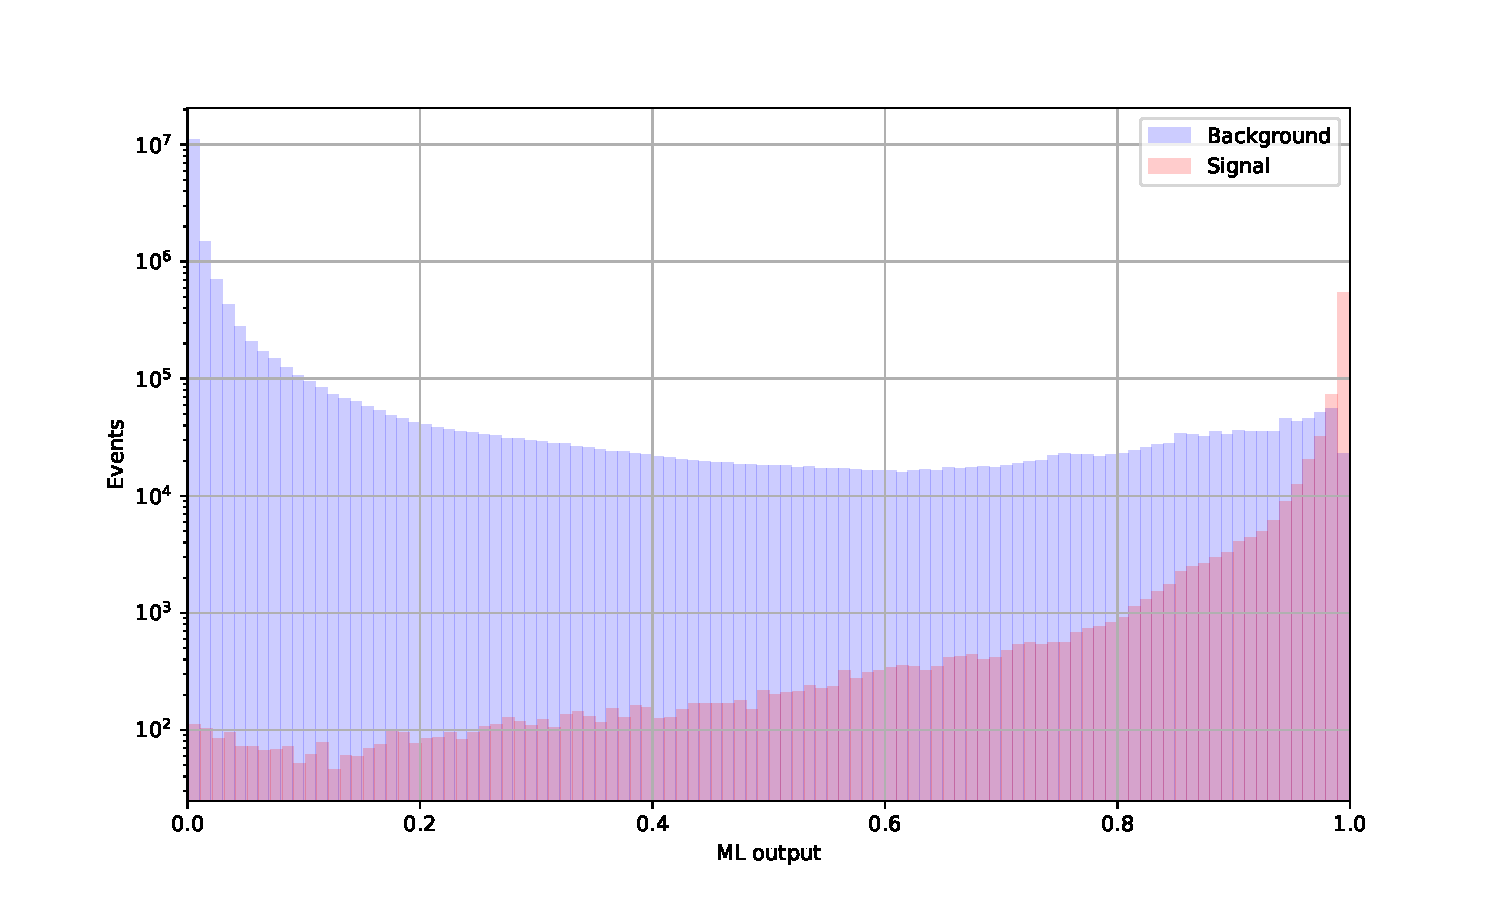
\includegraphics[width=\textwidth]{VAL_unscaled.pdf}
        \caption{No re-weighing MC events to expected events}
    \end{subfigure}
    \hfill
    \begin{subfigure}[b]{0.7\textwidth}
        \centering
        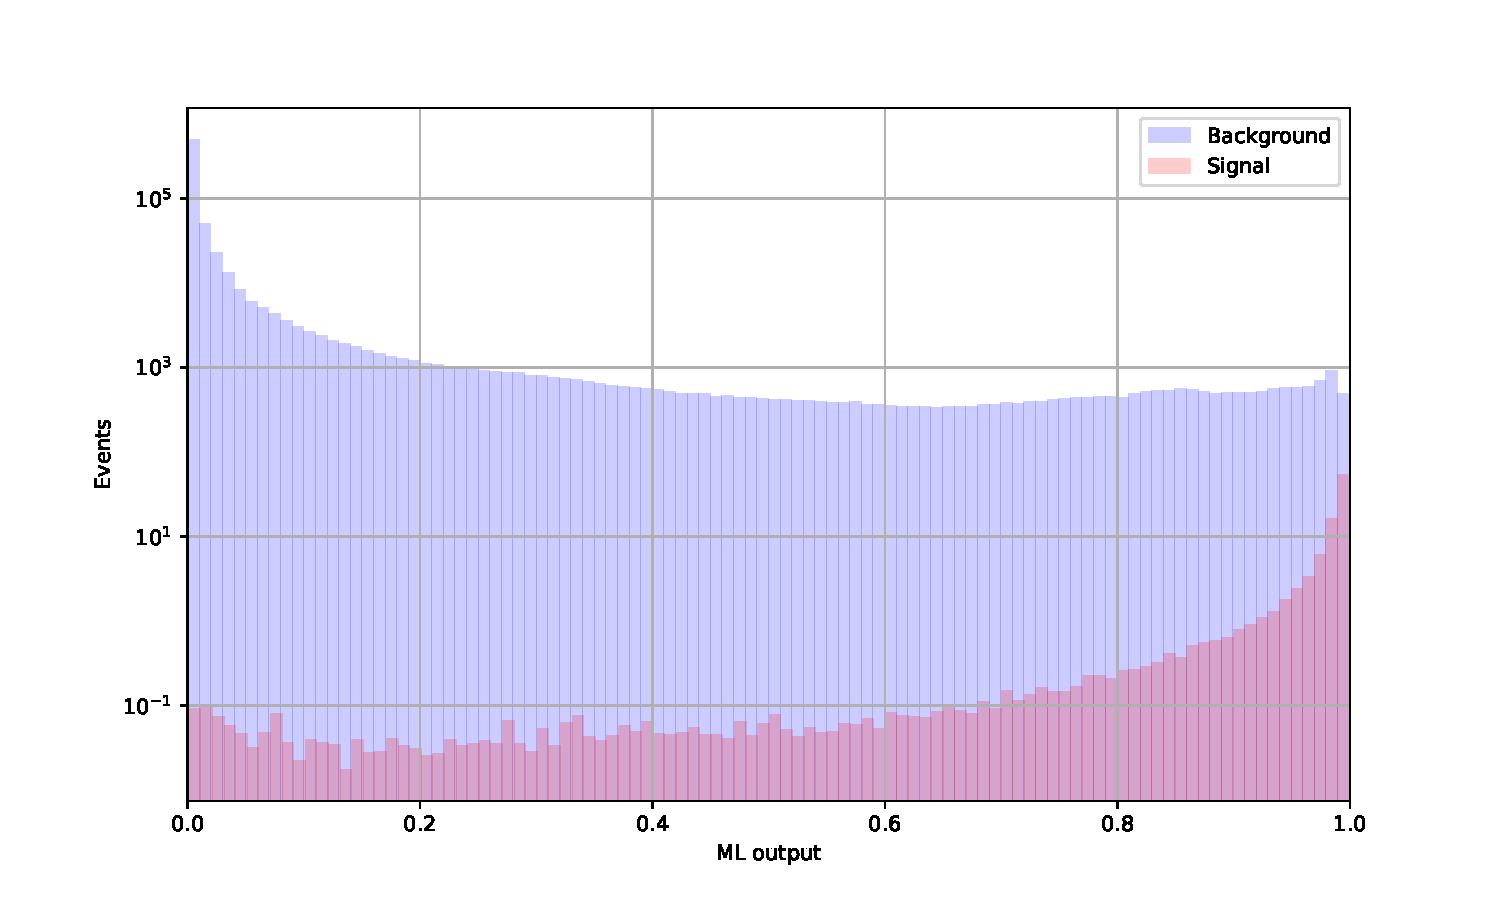
\includegraphics[width=\textwidth]{VAL.pdf}
        \caption{Re-weighing MC events to expected events}
    \end{subfigure}
    \caption[Validation plots illustration]{Illustration of the validation plots. Plot a) shows how the network learned a dataset whithout re-weighting events, while b) shows how it looks re-weighted.}\label{fig:VAL}
\end{figure}
\\It is standard practice to make fill the histrograms with semi-transparent colors, such that one can visualise the whole spectra for both background and signal. In this thesis we will use this, as well as validation plots where we divide the SM events into their respective background channels and fill them with opaque 
colors, while leaving the signal unfilled. We will in adition include real data points in the latter plots, to see how well SM simulations agree with the data. Ideally we want our data to not agree with the SM simulations when the network 
predicts a score close to one, as this discrepancy could be a hint of new physics.


\clearpage
\subsection{Significance plots}\label{sec:siggy}
To create signal regions which will be used for statistical analysis we will also look at significance plots. The way these plots work is by using Eq. (\ref{eq:exp_sig}) on the number of signal and background events that are presenent after making a cut on the ML output on the validation plots. 
As an example, in Figure \ref{fig:EXP_SIG} we se the re-weighted validation plot from the previous section, and we can calucate the expected significance by counting the number of signal and background events that have an ML score greater than 0.5, 0.6, 0.7, 0.8, 0.9 and 0.99 respectively.
\begin{figure}[!ht]
	\centering
    \begin{subfigure}[b]{0.7\textwidth}
        \centering
        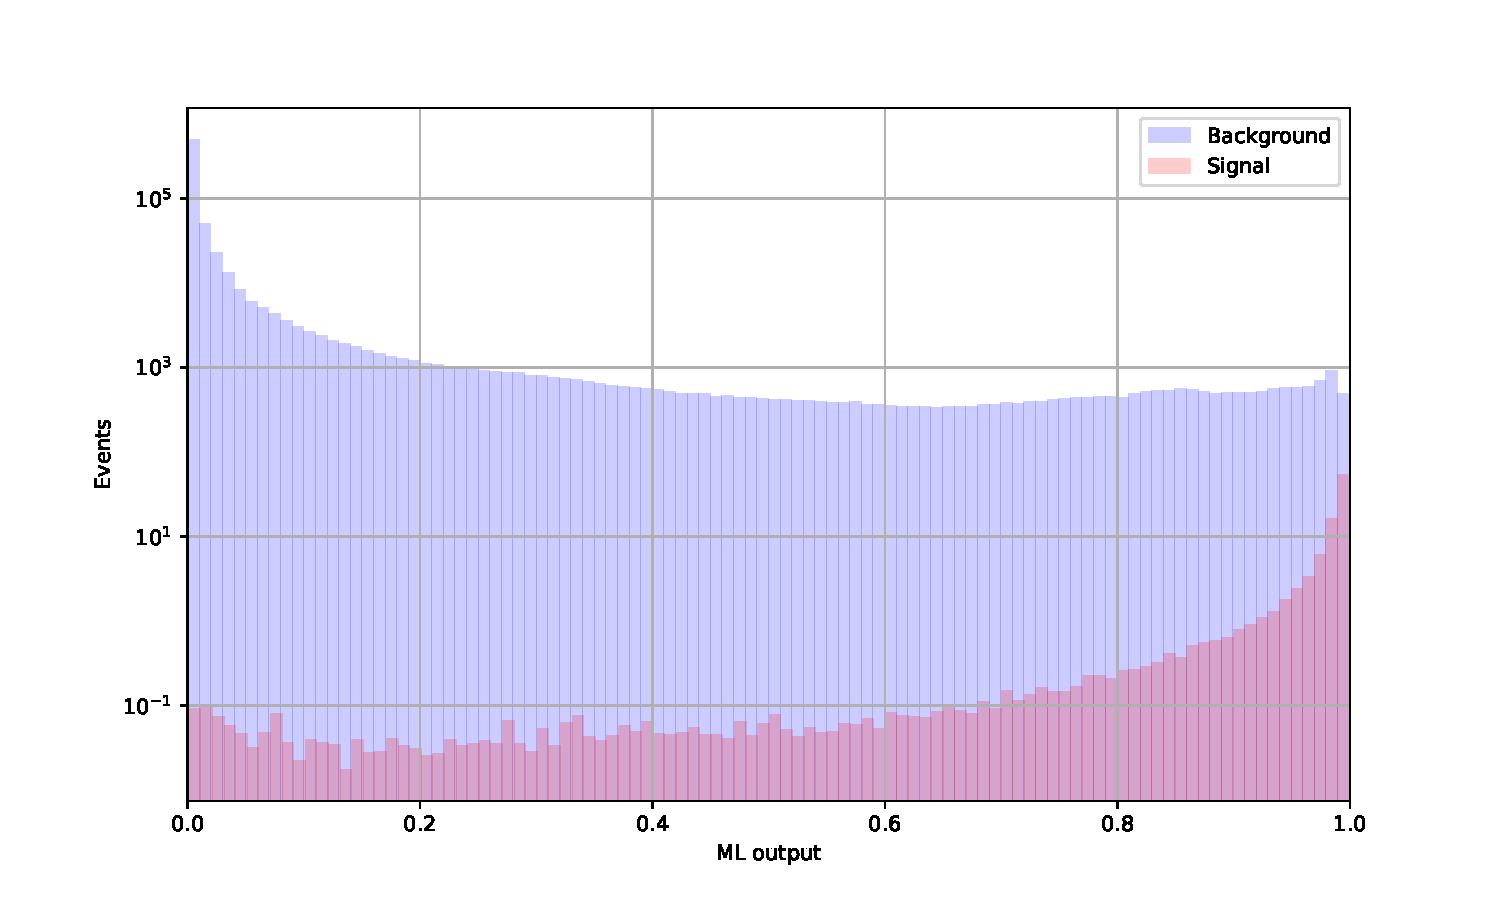
\includegraphics[width=\textwidth]{VAL.pdf}
    \end{subfigure}
    \hfill
    \begin{subfigure}[b]{0.7\textwidth}
        \centering
        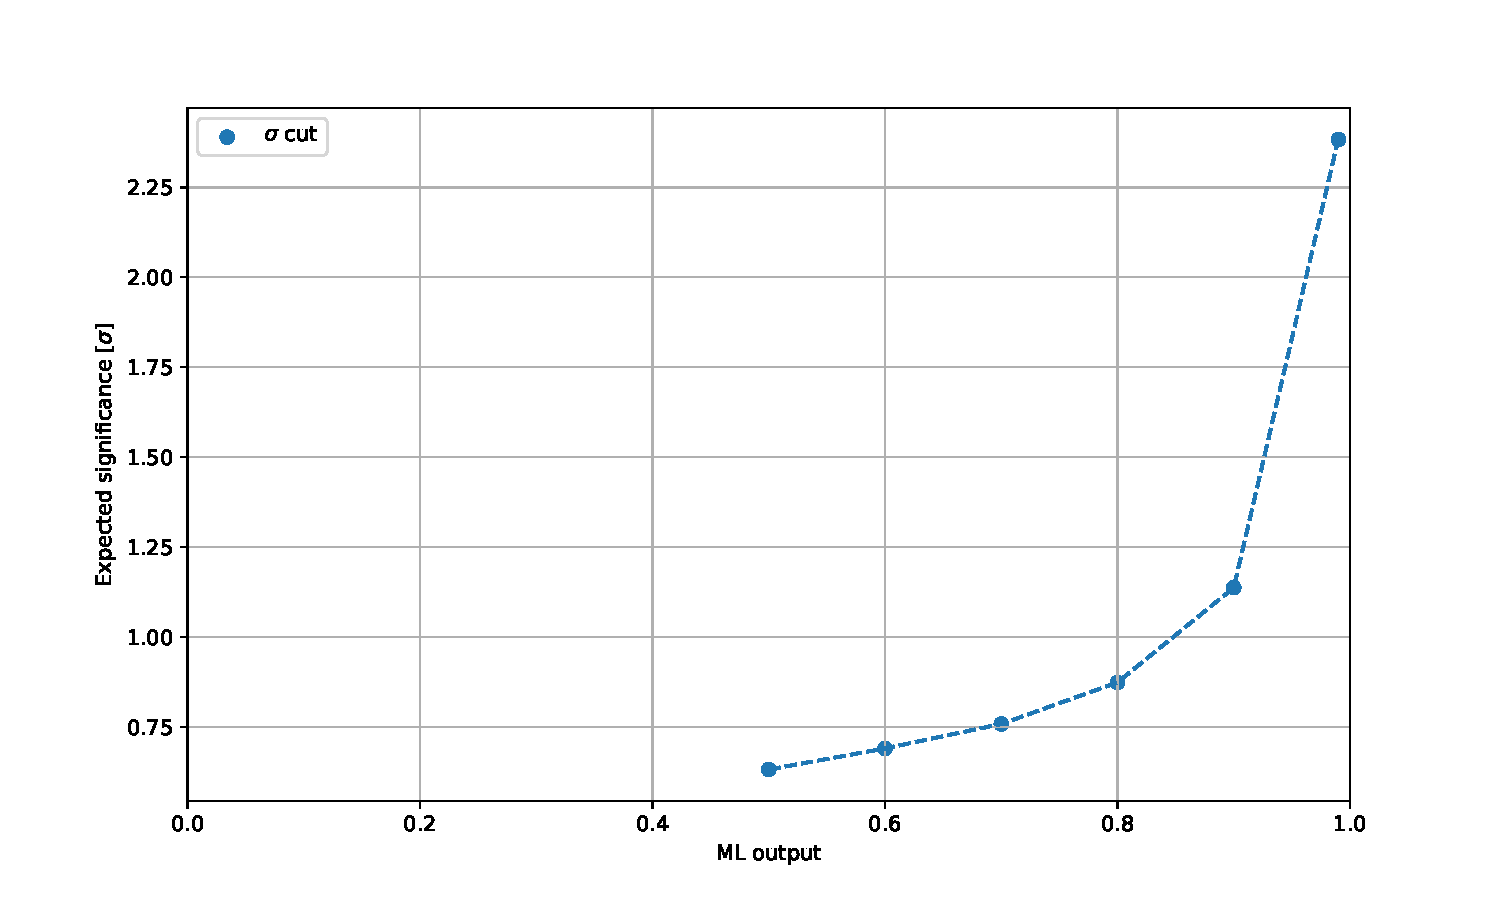
\includegraphics[width=\textwidth]{EXP_SIG.pdf}
    \end{subfigure}
    \caption[Significance plot illustration]{Plot showing the expected significance that is calculated from a) when making cuts on the ML output score. The dashed lines are to guide the eye.}\label{fig:EXP_SIG}
\end{figure}

\subsection{BDT and NN exclusive plots}\label{sec:feat}
\subsubsection{Feature importance}
For BDTs, as we can calculate which features had the most impact when splitting the data, we will also include feature importance plots. As the name states these plots tells us how important the features in the dataset were in the training to separate signal from background. As we are using the \verb|XGBoost| 
package when working with BDTs, we will use the inbuilt functions of the package to plot the feature importance. \\
\\When plotting the feature importance there are several metrics we can use to determine how important they are, for this thesis we will mainly look at 
\begin{itemize}
    \item Gain: which measures the relative contribution of a feature to the model's performance
    \item Weight: the number of times a feature appears on a tree to split the data
    \item Cover: the number of samples affected by the split with a feature
\end{itemize}
Where the first one is the standard used by \verb|XGBoost|.

\subsubsection{Metric and loss evolution}
For NNs we can plot how the metrics (AUC and binary accuracy) as well as the loss function change over the training epochs. We will plot these changes for both the training and testing set. Where the goal is that the metric and loss converge to the same point for the training and testing set.
\end{document}